
%----------------------------------------------------------------------------------------%
% START LaTeX preamble

% define document type, font and paper size
\documentclass[11pt,a4paper]{article}

%----------------------------------------------------------------------------------------%
% IMPORT LaTeX packages

\usepackage{inputenc}
\usepackage[ngerman, english]{babel}
\usepackage{csquotes}
\usepackage{amsmath}
\usepackage{amssymb}
\usepackage{amsfonts}
\usepackage{graphicx}
\usepackage{wrapfig}
\usepackage[margin=1.25in]{geometry}
\usepackage{pdfpages}
\usepackage{listings}
\usepackage{setspace}
\usepackage{systeme}
\usepackage{mdframed}

%----------------------------------------------------------------------------------------%
% SET user defined commands

\newcommand{\mathsym}[1]{{}}
\newcommand{\unicode}[1]{{}}

%----------------------------------------------------------------------------------------%
% IMPORT LaTeX packages to manange bibliography

% MLA, APA, or IEEE? - https://www.overleaf.com/learn/latex/Biblatex_citation_styles
\usepackage[style=apa]{biblatex}
\addbibresource{bibliography.bib}

%----------------------------------------------------------------------------------------%
% DEFINE header values

% define the cover page values
\title
{
    Assessed exercise 02\\
    49th CIDTEC
}
\author
{
    Antonio Osamu Katagiri Tanaka \\
    A01212611
}
\date{\today}

%----------------------------------------------------------------------------------------%
% USER-DEFINED commands

% Keywords command
\providecommand{\keywords}[1]
{
    \\
    \\
    \small
    \textbf{\textit{Keywords:}} #1
}

%----------------------------------------------------------------------------------------%

\begin{document}

%----------------------------------------------------------------------------------------%
% CREATE the 1st page (cover page)

%uncomment
%\maketitle

%----------------------------------------------------------------------------------------%
% DEFINE the abstract text & keywords

%uncomment
%\begin{abstract}
%    \emph
%    {
%        Lorem ipsum dolor sit amet, consectetur adipiscing elit, sed do eiusmod tempor incididunt ut labore et dolore magna aliqua. Ut enim ad minim veniam, quis nostrud exercitation ullamco laboris nisi ut aliquip ex ea commodo consequat. Duis aute irure dolor in reprehenderit in voluptate velit esse cillum dolore eu fugiat nulla pariatur. Excepteur sint occaecat cupidatat non proident, sunt in culpa qui officia deserunt mollit anim id est laborum.
%    }
%    \keywords{Lorem, ipsum, dolor, sit, amet}
%\end{abstract}

%----------------------------------------------------------------------------------------%
\clearpage

%----------------------------------------------------------------------------------------%
% CREATE a table of contents in a new page

%uncomment
%\tableofcontents
\clearpage

%----------------------------------------------------------------------------------------%
% CREATE a list of figures and a list of tables in a new page

%uncomment
%\listoffigures
%\listoftables
\clearpage

%----------------------------------------------------------------------------------------%
% DOCUMENT body starts here
\includepdf[pages=-]{Chap10_1}
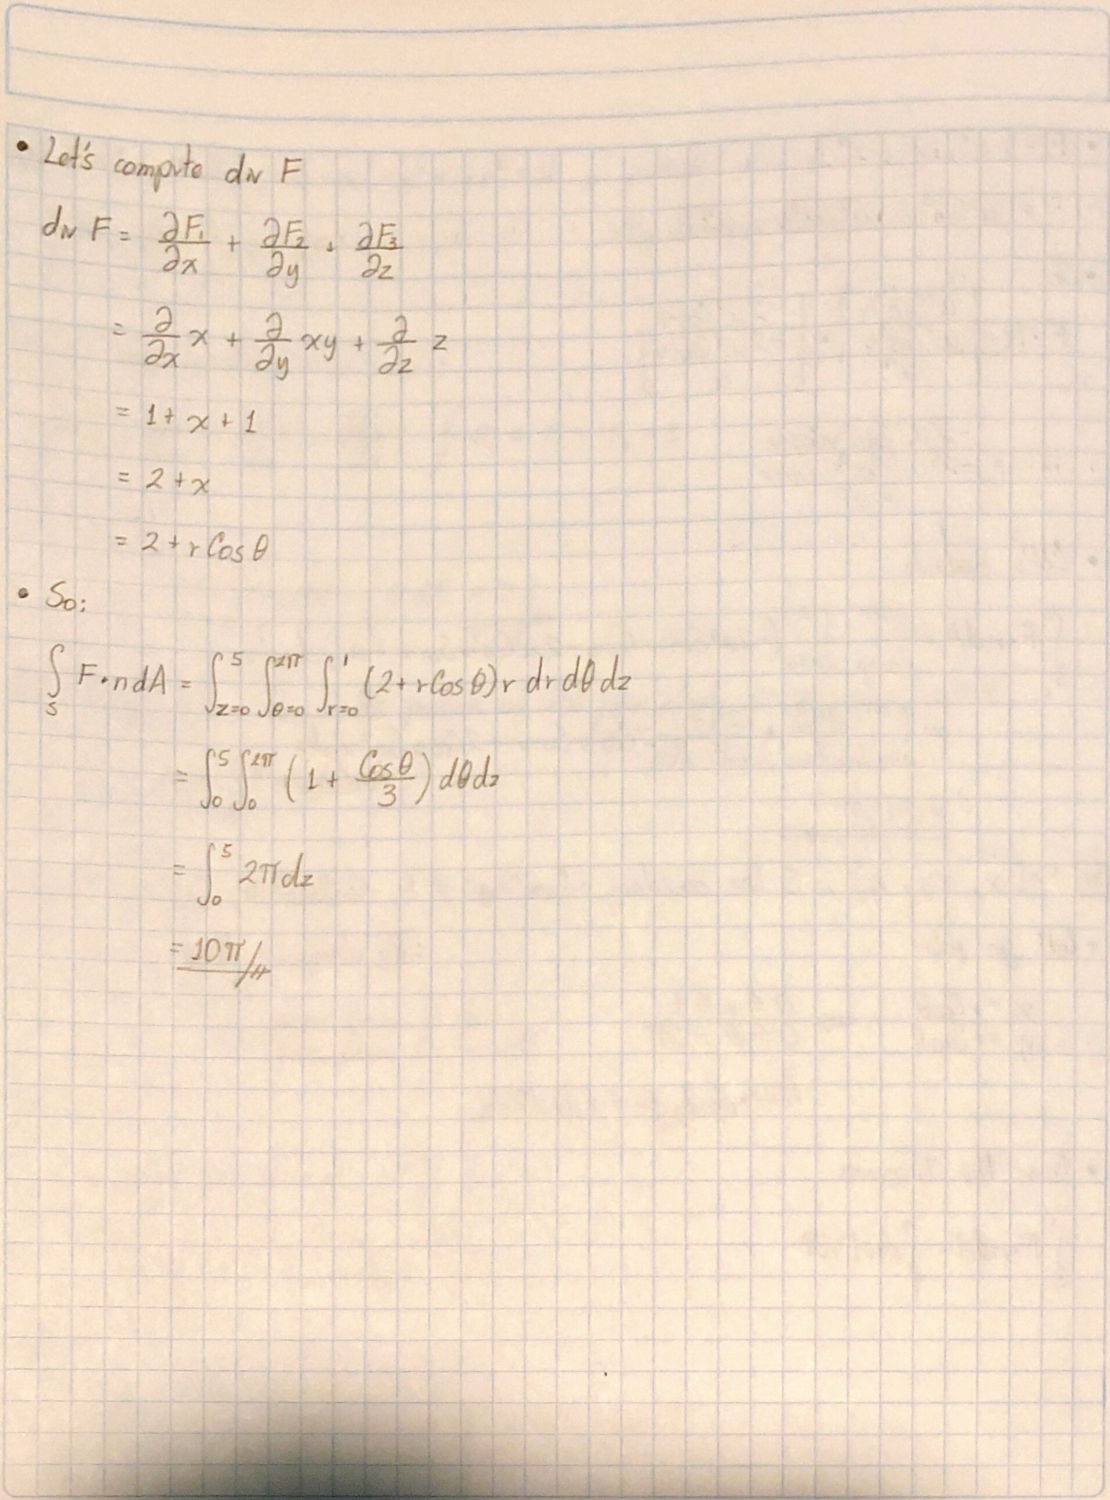
\includepdf[pages=-]{Chap10_2}

%----------------------------------------------------------------------------------------%

\end{document}

%----------------------------------------------------------------------------------------%
